% TeamSync AI --- IEEEtran paper source.
% Compiled from IEEE_PAPER_REPORT.md; every number here matches that report
% and the committed evaluation scripts in ai-service/eval/.
%
% Compile (twice, to resolve references/figure numbers):
%   pdflatex paper.tex && pdflatex paper.tex
% Or upload this file plus docs/paper_figures/*.pdf to Overleaf.
%
% NOTE ON AUTHORSHIP: the \author block below is a placeholder. Replace with
% the real author list and affiliation before submission -- do not submit
% with placeholder names.

\documentclass[conference]{IEEEtran}
\usepackage{graphicx}
\usepackage{booktabs}
\usepackage{amsmath}
\usepackage{listings}
\usepackage{xcolor}
\usepackage{hyperref}
\usepackage{url}

\lstset{
  basicstyle=\ttfamily\footnotesize,
  breaklines=true,
  frame=single,
  columns=fullflexible,
  backgroundcolor=\color{gray!8}
}

\begin{document}

\title{TeamSync AI: Explainable, Graph-Grounded Multi-Agent Project Intelligence}

% PLACEHOLDER -- replace before submission.
\author{
  \IEEEauthorblockN{Author Name(s)}
  \IEEEauthorblockA{Department/Affiliation \\ Institution \\ City, Country \\ email@institution.edu}
}

\maketitle

\begin{abstract}
Conventional project-management tools surface current state but not predictive,
evidence-linked risk, and naive attempts to add large-language-model (LLM) analysis
inherit the LLM's cost, non-determinism, and unverifiable justifications. We present
TeamSync AI, a project-intelligence system built on \emph{graph-grounded agent
prompting}: project state is compiled into a typed knowledge graph, six categories of
team coordination risk are computed as deterministic graph invariants (critical path,
articulation points, weighted degree, community structure), and a language model is
shown only the minimal witness subgraph of one already-computed finding to narrate it
in prose -- never to decide whether the risk exists. Every citation the model emits is
mechanically checked against the witness subgraph and stripped if unverifiable. This
design yields two measured properties: prompt cost that scales with the number of
anomalies rather than project size (measured 1.47$\times$ token growth for a
154$\times$ larger project; a 487$\times$ reduction against naive full-dataset
prompting at 2{,}003 tasks), and evidence grounding that is enforced rather than
requested (200/200 fabricated citations correctly stripped in trial). On a held-out,
project-level split of a real 458{,}232-issue Jira dataset (TAWOS, 22 unseen
projects), the same graph, projected forward from work completed so far, warns of
sprints that will finish late while they are still running: AUC 0.792 at the halfway
point and 0.874 at three-quarters, improving on flagging every sprint by F1 +0.050
(95\% CI [+0.006, +0.094]) and +0.099 ([+0.049, +0.148]), both $p < 0.001$. Evaluated
after the deadline instead, the untuned, zero-parameter rule reaches F1 = 0.712 (95\%
bootstrap CI [0.610, 0.814]) where a logistic-regression model that reached
cross-validated F1 = 0.816 on the tuning split falls to 0.593; a paired test cannot
separate the two ($p = 0.78$), so we claim not that the simple rule predicts better,
but that the tuned model's advantage did not cross project boundaries. Three
independent attempts to improve on the simple rule with more sophisticated methods all
failed or backfired on held-out data, a set of negative results we report in full
because they are what make the headline claim credible. A controlled ablation further shows the token-efficient graph architecture
matches or exceeds naive full-dataset LLM prompting on detection accuracy (F1 1.000
vs.\ 0.947), so the efficiency gain does not trade away correctness.
\end{abstract}

\begin{IEEEkeywords}
explainable AI, multi-agent systems, knowledge graphs, large language models, project
management, software risk prediction, evidence grounding
\end{IEEEkeywords}

\section{Introduction}

Teams using conventional project-management tools (Jira, Linear, Asana, Monday.com)
run into four compounding failures. First, risk is detected late: tools show current
state, not risk trajectory, so a silently overloaded engineer or a slipping
critical-path task becomes visible only after the damage. Second, warnings are opaque:
when a tool does flag something ``at risk,'' it rarely shows which evidence produced
that verdict, so a manager can neither act on it nor challenge it. Third, signals are
siloed: no single view reveals a cross-cutting risk such as ``the only person who
understands this component is also unresponsive and on the critical path.'' Fourth,
naive attempts to bolt an LLM onto this problem introduce new failure modes: feeding
raw project data to a language model is expensive (cost scales with project size),
non-deterministic (identical input can yield different verdicts), and produces
justifications that cannot be independently checked.

This raises the question we address: \emph{can a system detect coordination risk
early, explain it with verifiable evidence, and remain cheap enough to run
continuously, without trading away accuracy for that cheapness?}

Our answer inverts the typical ``LLM finds the problem'' architecture. Rather than
asking a language model to search raw project data for risk, we (1) compile project
state into a typed knowledge graph built entirely from data the product already
stores; (2) compute every risk category as a deterministic graph algorithm, at zero
token cost and zero randomness; (3) extract a small \emph{witness subgraph} around
each detected anomaly; (4) give the LLM only that witness subgraph and ask it to
\emph{narrate} the already-computed finding, never to decide whether it exists; and
(5) mechanically verify every citation the model emits against the witness subgraph,
discarding anything that does not resolve to a real node. Every agent additionally
carries a deterministic rule-based fallback sharing the exact same output schema, so
the system is fully functional with no LLM configured at all.

\textbf{Contributions.} (i) \emph{Graph-grounded agent prompting}, an architecture in
which risk computation and risk explanation are cleanly separated, with the language
model restricted to the latter. (ii) A measured demonstration that this separation
makes prompt cost scale with the number of anomalies rather than with project size --
a 487$\times$ reduction against naive prompting at scale. (iii) A mechanical
evidence-grounding check that converts ``the model was asked to cite sources'' into
``every surviving citation is verifiably real,'' rather than relying on prompt
compliance. (iv) A held-out, real-world evaluation, including three reported negative
results, showing that a zero-parameter deterministic rule matches a tuned learned
model on unseen data -- the two cannot be separated by a paired test, while the
learned model's cross-validated advantage does not survive the project boundary -- and
a controlled ablation showing this efficiency does not cost detection accuracy.
(v) A pre-registered mid-sprint evaluation on the same held-out projects, in which the
graph projected forward from completed work identifies sprints that will finish late at
their halfway point (AUC 0.792, and 0.874 at three-quarters), moving the warning to a
point where it can still change the outcome.

The remainder of this paper is organized as follows. Section~II positions this work
against related tooling and techniques. Section~III describes the system
architecture. Section~IV details the graph-grounded prompting mechanism, the central
contribution. Section~V describes the multi-agent design. Section~VI describes the
experimental setup. Section~VII reports results. Section~VIII discusses the findings,
including the negative results and their implications. Section~IX states threats to
validity. Section~X concludes.

\section{Related Work}

We position this work against three groups of prior work, summarized in
Table~\ref{tab:related}.

\textbf{Traditional project-management tools} (Jira, Linear, Asana, Monday.com)
surface current task and milestone state but not predictive, evidence-linked risk;
where an ``at risk'' flag exists, its underlying evidence is not exposed.

\textbf{LLM-based multi-agent systems} such as MetaGPT~\cite{metagpt},
ChatDev~\cite{chatdev}, and benchmarks such as AgentBench~\cite{agentbench} and
techniques such as ReAct~\cite{react} optimize for task completion by language-model
agents. None of these separate a deterministic, checkable computation from a
narration step in the way this system does; the model's own reasoning is typically
the source of the answer, not merely its narrator.

\textbf{Explainable AI (XAI) in software engineering}, including SHAP~\cite{shap},
LIME~\cite{lime}, and model-agnostic XAI techniques applied to defect
prediction~\cite{jiarpakdee}, explain a \emph{learned model's} prediction after the
fact. In our system the underlying computation is a deterministic graph invariant
that needs no post-hoc explanation in the statistical sense; the language model's
sole role is narration under a mechanically enforced citation constraint. This is a
difference in kind, not merely in implementation.

\textbf{Retrieval-grounded generation}, such as retrieval-augmented
generation~\cite{rag} and the broader literature on LLM hallucination~\cite{hallucination-survey},
grounds generation by conditioning on retrieved text. Our system instead grounds in
a \emph{computed, typed graph} and verifies citations against it \emph{after}
generation, rather than relying on retrieval alone to prevent fabrication.

No single comparator combines: specialist multi-agent decomposition, graph-computed
(not LLM-inferred) risk, mechanically enforced evidence grounding, a deterministic
fallback sharing an identical output schema, and a held-out real-world evaluation
that reports negative results alongside positive ones.

\begin{table}[t]
\caption{Related work positioning}
\label{tab:related}
\centering
\begin{tabular}{p{1.6cm}p{2.7cm}p{3.2cm}}
\toprule
\textbf{Group} & \textbf{Examples} & \textbf{What they lack} \\
\midrule
PM tools & Jira, Linear, Asana & Predictive, evidence-linked risk \\
LLM multi-agent & MetaGPT, ChatDev, AgentBench, ReAct & Deterministic, checkable risk computation \\
XAI in SE & SHAP, LIME, defect-prediction XAI & Explaining a computed invariant, not a learned model \\
Retrieval grounding & RAG, hallucination surveys & Post-hoc mechanical citation verification \\
\bottomrule
\end{tabular}
\end{table}

\section{System Architecture}

TeamSync AI comprises three independently deployable services (Fig.~\ref{fig:topology}):
a Next.js frontend; a FastAPI core API handling authentication, CRUD operations,
multi-tenancy, and persistence; and a FastAPI AI service hosting the knowledge-graph
engine and the multi-agent analysis pipeline. The AI service is the locus of the
paper's contribution and degrades gracefully to a fully deterministic path when no
LLM is configured.

\begin{figure}[t]
\centering
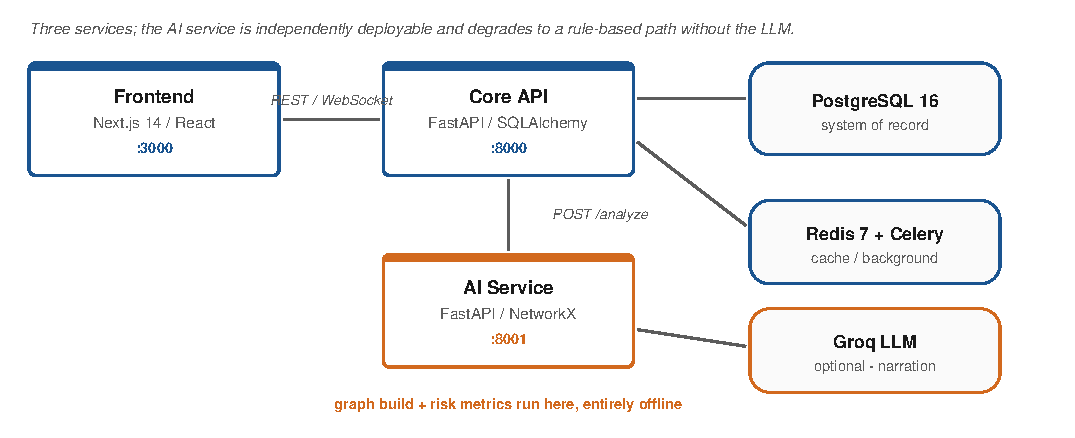
\includegraphics[width=\columnwidth]{docs/paper_figures/fig0_topology.pdf}
\caption{Service topology. The AI service holds the graph engine and degrades to a
rule-based path with no LLM configured.}
\label{fig:topology}
\end{figure}

\subsection{Knowledge Graph Schema}

The graph has five node types --- Person, Task, Milestone, Project, Component --- and
nine edge types, all derived from tables the product already stores, requiring no new
data collection: \texttt{ASSIGNED\_TO} (person to task, weighted by story points),
\texttt{REPORTED}, \texttt{BLOCKS} (task dependency), \texttt{SUBTASK\_OF},
\texttt{PART\_OF} (task to milestone), \texttt{COMMENTED\_ON}, \texttt{MEMBER\_OF}
(person to project), \texttt{TOUCHES} (task to component), and \texttt{KNOWS}
(a person-to-component edge derived by composing \texttt{ASSIGNED\_TO} with
\texttt{TOUCHES}).

\subsection{The Analysis Pipeline}

Fig.~\ref{fig:pipeline} shows the pipeline. Project data is compiled into the
knowledge graph (NetworkX~\cite{networkx}); six risk categories are computed as
graph algorithms (Table~\ref{tab:risks}); a bounded witness subgraph is extracted
around each anomaly; and only that subgraph crosses into the LLM narration layer.
Risk \emph{scores} never depend on the language model -- only the accompanying prose
does.

\begin{figure}[t]
\centering
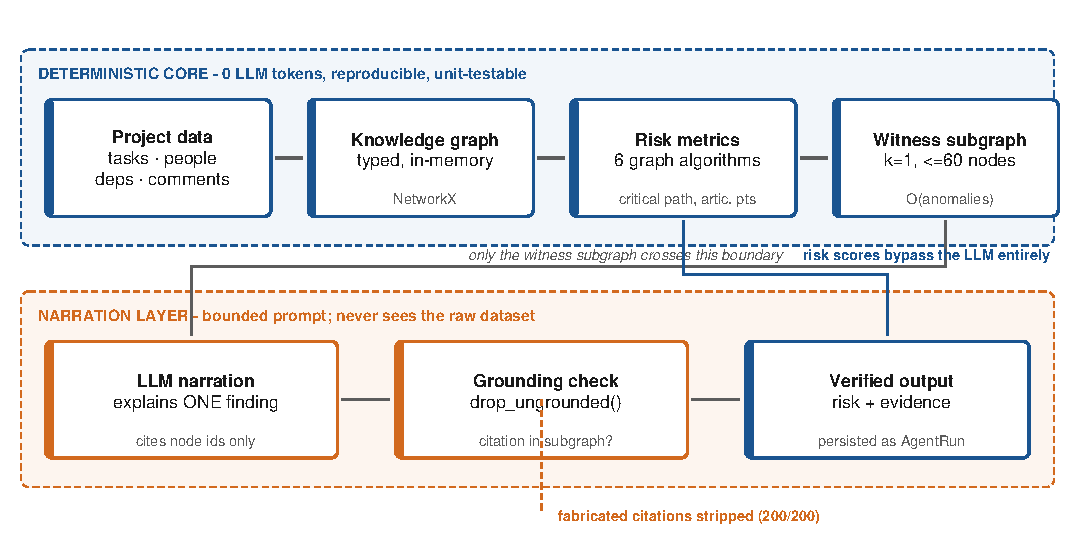
\includegraphics[width=\columnwidth]{docs/paper_figures/fig1_architecture.pdf}
\caption{The analysis pipeline. The deterministic core (left) computes risk at zero
token cost; only a bounded witness subgraph crosses into the narration layer
(right), and every citation is checked before the output is returned.}
\label{fig:pipeline}
\end{figure}

\begin{table}[t]
\caption{The six risk types as graph algorithms}
\label{tab:risks}
\centering
\begin{tabular}{p{2.0cm}p{4.0cm}p{1.5cm}}
\toprule
\textbf{Risk type} & \textbf{Graph computation} & \textbf{Threshold} \\
\midrule
Dependency (critical path) & Longest path through the \texttt{BLOCKS} DAG & $\geq 0.25$ \\
Dependency concentration & Betweenness centrality of task nodes & --- \\
Knowledge / SPOF & Articulation points, Person--Component graph & $\geq 2$ tasks \\
Workload & Weighted degree over \texttt{ASSIGNED\_TO} & $\geq 1.5\times$ \\
Coordination & Community structure / isolated members & --- \\
Silent member & \texttt{COMMENTED\_ON} $\div$ \texttt{ASSIGNED\_TO} degree & $\geq 0.30$ \\
Delay & Open tasks past due date & $\geq 0.10$ \\
\bottomrule
\end{tabular}
\end{table}

A correctness benefit followed directly from building the graph: the pre-existing
dependency-creation API rejected only direct self-loops, so a three-hop circular
dependency ($A \to B \to C \to A$) was creatable through the interface. Cycle
detection over the \texttt{BLOCKS} edge type catches such cycles for free once the
graph exists.

\section{Graph-Grounded Agent Prompting}

This section details the paper's central contribution: separating deterministic risk
\emph{computation} from LLM-based risk \emph{narration}, and mechanically enforcing
that separation.

\subsection{Witness Subgraph Selection}

The witness subgraph is extracted with a one-hop neighborhood expansion around each
anomaly's seed nodes, capped at eight neighbors per seed and sixty nodes total; seed
nodes always survive truncation. The per-seed neighbor cap is the mechanism that
makes prompt cost independent of project size: without it, a high-degree node (for
example, a person with hundreds of open tasks) would pull its entire neighborhood
into the prompt, and prompt size would once again scale with project size rather than
anomaly count. We discovered this precisely by measuring it: an early, uncapped
implementation showed 4.31$\times$ witness-subgraph growth from 50 to 2{,}000 tasks;
adding the per-seed cap reduced this to 1.007$\times$. Serialization is columnar
rather than JSON, stating each field name once per block header rather than once per
row, which accounts for most of the remaining token saving once the node set itself
is already small.

\subsection{Evidence Grounding}

Every evidence citation an agent emits carries a \texttt{reference\_id}. After
generation, a grounding check computes the set of valid node identifiers from the
witness subgraph and discards any citation whose \texttt{reference\_id} is not a
member of that set. This is enforced as a checked invariant on the output, not
requested as a prompt instruction -- the distinction between ``the model was told to
cite evidence'' and ``every surviving citation is verifiably real.'' In 200 trials in
which fabricated references were synthetically injected into agent output, all 200
were correctly identified and stripped.

A related implementation defect illustrates why this needs to be a post-generation
check rather than a prompt-level assumption: an early version of the grounding logic
treated an \emph{empty} findings list identically to \emph{no} filter being applied
(a falsy-empty-list bug), which would have silently allowed every citation through
precisely when nothing should have been grounded. This was caught before being
relied upon and fixed to distinguish ``grounded against nothing'' from ``grounding
disabled.''

\subsection{Efficiency Result}

Table~\ref{tab:tokens} and Fig.~\ref{fig:tokens} report the token-scaling
measurement. As project size grows 154$\times$ (13 to 2{,}003 tasks), prompt size
under graph-grounded prompting grows only 1.47$\times$ (266 to 390 tokens), while
naive full-dataset prompting grows linearly to 189{,}834 tokens at the same
size -- a 487$\times$ gap at the largest measured size.

\begin{table}[t]
\caption{Prompt token scaling: graph-grounded vs.\ naive prompting}
\label{tab:tokens}
\centering
\begin{tabular}{rrrr}
\toprule
\textbf{Tasks} & \textbf{Graph} & \textbf{Naive} & \textbf{Ratio} \\
\midrule
13 & 266 & 1{,}050 & 3.9$\times$ \\
53 & 386 & 4{,}695 & 12.2$\times$ \\
203 & 389 & 18{,}901 & 48.6$\times$ \\
1{,}003 & 389 & 94{,}724 & 243.5$\times$ \\
\textbf{2{,}003} & \textbf{390} & \textbf{189{,}834} & \textbf{486.8$\times$} \\
\bottomrule
\end{tabular}
\end{table}

\begin{figure}[t]
\centering
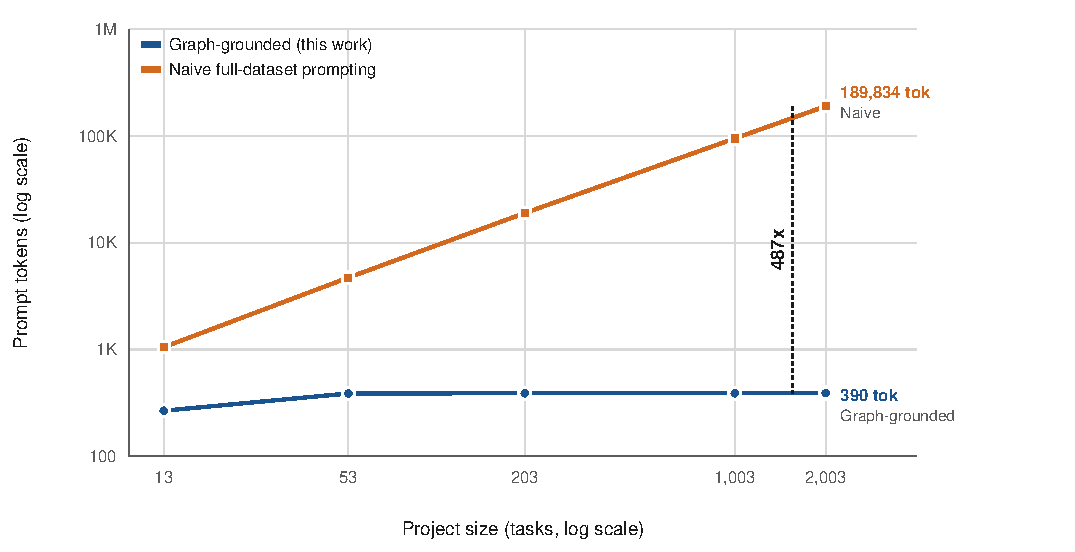
\includegraphics[width=\columnwidth]{docs/paper_figures/fig2_token_scaling.pdf}
\caption{Prompt cost against project size (log--log). Graph-grounded prompting is
effectively flat; naive prompting grows linearly.}
\label{fig:tokens}
\end{figure}

Crucially, this efficiency gain does not trade away detection accuracy, as
Section~VII-D demonstrates with a controlled, naive-vs-graph ablation.

\section{Multi-Agent Design}

The pipeline follows a coordinator pattern: a coordinator invokes three specialist
agents in parallel (Planning, Progress, Workload), a risk aggregator combines the six
graph-computed scores, and a recommendation generator proposes prioritized actions
(Table~\ref{tab:agents}). Two further agents (Meeting Intelligence, Communication
Intelligence) and a multi-agent review consensus mechanism are architecturally
designed but deliberately deferred, because the product does not yet ingest the
transcript or chat/email data those agents require -- an explicit scoping decision,
not a hidden gap.

\begin{table}[t]
\caption{Agent roster}
\label{tab:agents}
\centering
\begin{tabular}{p{1.6cm}p{2.9cm}p{2.1cm}}
\toprule
\textbf{Agent} & \textbf{Reads} & \textbf{Produces} \\
\midrule
Planning & Milestones, capacity, graph metrics & Sprint readiness, capacity gaps \\
Progress & Tasks, velocity, graph metrics & Velocity trend, stalled work \\
Workload & Assignments, graph metrics & Overload, single points of failure \\
Risk & Six graph-computed scores & Aggregated scores + evidence \\
Recommendation & Risk + specialist outputs & Prioritized actions \\
\bottomrule
\end{tabular}
\end{table}

Every agent, whether LLM-backed or running its deterministic fallback, returns one
shared output schema:

\begin{lstlisting}
AgentOutput:
  summary: str
  risk_level: low | medium | high | critical
  confidence: float in [0, 1]
  signals: [{name, value, weight}]
  evidence: [{source, reference_id,
              excerpt, relevance}]
  recommendations: [{type, title,
              description, reasoning,
              priority, confidence}]
  next_action: str
  metadata: dict  # fallback: bool
\end{lstlisting}

The rule-based fallback for each agent is deterministic and independent of the LLM
path, so a failed or absent language-model call degrades the pipeline gracefully
rather than crashing it -- the entire pipeline, including risk computation, evidence
citation, and recommendation generation, functions correctly with no LLM configured
at all.

\section{Experimental Setup}

\subsection{Real-World Dataset: TAWOS}

We evaluate against TAWOS~\cite{tawos}, a public dataset of 458{,}232 real Jira
issues drawn from 39 open-source projects across 12 Jira repositories, released
under Apache License 2.0. TAWOS carries no \texttt{due\_date} field, so we define a
sprint as \emph{delayed} when at least 30\% of its issues remained unresolved at
sprint end. Restricting to closed sprints with a recorded end date and at least 15
issues yields 987 eligible sprints across 31 projects (58.8\% positive rate).

Because every issue in an archival dataset is long since resolved, using current
status directly would leak future information into a retrospective label. We instead
reconstruct each task's state \emph{as of sprint end} and evaluate graph metrics with
the clock set to one day after sprint end, so that only information available at the
time would have been available to the system.

\subsection{Split Discipline}

We split by \emph{project}, not by sprint: 9 projects (717 sprints) for tuning and
22 projects (270 sprints, 48.9\% positive) held out entirely. Splitting by project
prevents a single team's Jira conventions from leaking across the tuning/held-out
boundary. The held-out set was evaluated exactly once, after all tuning decisions
were frozen.

\subsection{Synthetic Scenarios}

For implementation-correctness checks independent of any external dataset, we also
generate 180 synthetic scenarios (90 positive, 90 negative; 30 per risk type) with a
deterministically injected anomaly, so ground truth is known by construction. These
scenarios also underlie the ablation in Section~VII-D.

\section{Results}

\subsection{Synthetic Detection Correctness}

On the 180 synthetic scenarios, the deterministic detectors achieve precision,
recall, F1, and accuracy of 1.00 each (stable across four additional random seeds,
1{,}200 further trials). We emphasize the correct interpretation of this number: for
deterministic threshold code evaluated on unambiguous synthetic inputs, 100\% is the
\emph{expected} outcome of implementation correctness -- equivalent to all unit tests
passing -- and is not evidence of real-world generalization. The genuinely
falsifiable check is a threshold-boundary sweep, verifying that each detector flips
exactly at its documented threshold (e.g., the overdue-ratio detector flips at
exactly 0.10; the silent-ratio detector flips between 0.20 and 0.30, bracketing its
documented 0.30 threshold).

\subsection{Real-World Result: TAWOS}

On all 987 sprints with default, untuned parameters, the graph-computed delay rule
achieves precision 0.630, recall 1.000, F1 0.773, and accuracy 0.655, against a
story-point-median baseline's precision 0.545, recall 0.386, F1 0.452, and accuracy
0.450.

\textbf{Mid-sprint prediction.} The evaluation that matters to a practitioner asks
whether a sprint is in trouble while it is still running. We rebuild each held-out
sprint as it stood at a checkpoint -- only issues created by then exist, only issues
resolved by then are done, and the clock is set to that moment -- and project the share
of scope that will remain unfinished at the deadline, raising a delay risk from the
severity cutoffs already used elsewhere in the system. The checkpoints (50\%, 75\%), the
prediction, and the cutoffs were fixed before the held-out projects were touched, and
nothing was tuned for this experiment. On the 270 held-out sprints (48.9\% of which
finished late), the rule achieves F1 0.706 (precision 0.581, recall 0.902) at the
halfway point and F1 0.756 (precision 0.623, recall 0.962) at three-quarters, against
0.657 for flagging every sprint; paired by sprint, the differences are +0.050 (95\% CI
[+0.006, +0.094]) and +0.099 ([+0.049, +0.148]), exact McNemar $p < 0.001$ in both
cases. Ranked by the projected unfinished share, AUC is 0.792 and 0.874. We note
explicitly that a simple open-work-share baseline ranks the same sprints as well (AUC
0.802 and 0.881): the projection's contribution is an early warning carrying the same
verifiable evidence as every other finding, not superior ranking.

\textbf{Sprint-end evaluation.} Evaluated after the deadline instead, on the same
270-sprint held-out set, the untuned zero-parameter rule achieves precision 0.552,
recall 1.000, F1 0.712, against a composite logistic-regression model (tuned via
three-fold group cross-validation on the training split) achieving precision 0.620,
recall 0.568, F1 0.593, AUC 0.658 (Fig.~\ref{fig:holdout}). The perfect recall here is
structural rather than skillful: at sprint end, a delayed sprint is by definition one
with work unfinished past the due date, which is precisely the condition the rule
tests. What the comparison does show is the operating point -- over-flagging roughly
half the on-time sprints in exchange for missing none -- appropriate when a missed risk
is costlier than a dismissible false alarm.

\begin{figure}[t]
\centering
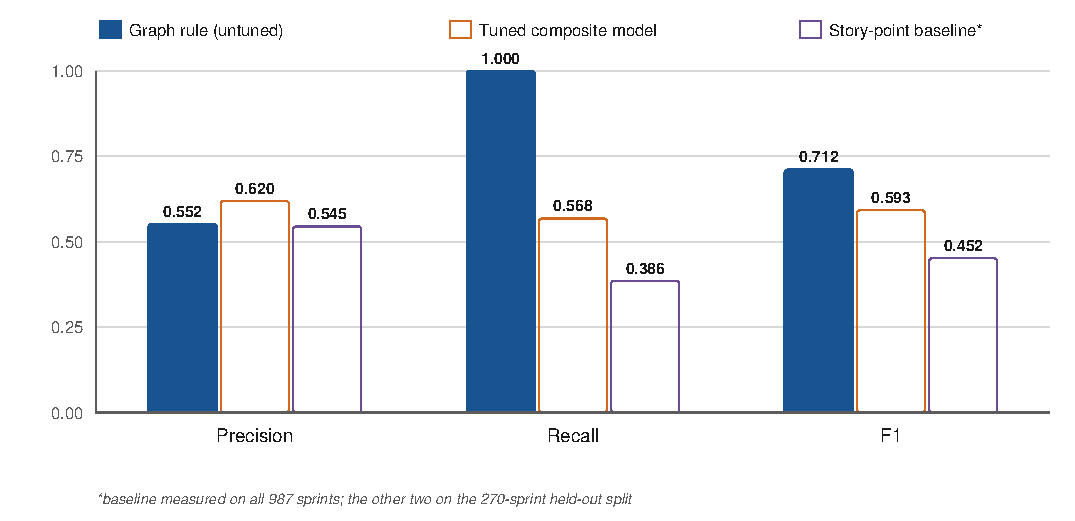
\includegraphics[width=\columnwidth]{docs/paper_figures/fig3_holdout_tawos.pdf}
\caption{Held-out precision/recall/F1 for the untuned graph rule, a tuned composite
model, and the story-point baseline.}
\label{fig:holdout}
\end{figure}

\textbf{Bootstrap confidence interval.} To quantify the stability of the F1 = 0.712
point estimate, we performed a cluster bootstrap over the 22 held-out projects (2{,}000
resamples, resampling projects with replacement and pooling their sprints), rather
than resampling individual sprints, because sprints within one project are
correlated -- the same reasoning that motivated the project-level split itself. The
resulting 95\% confidence interval is F1 $\in [0.610, 0.814]$, precision $\in [0.438,
0.686]$, and accuracy $\in [0.517, 0.719]$. Recall's interval is degenerate at
$[1.000, 1.000]$: every held-out project has zero false negatives under the untuned
rule, so no resample can introduce one either; this is a genuine property of the
data, not a bootstrap artifact, and we report it as such rather than obscuring it.
Comparing that interval to the composite model's point estimate would not be a test,
so we ran paired ones on the same sprints: against the composite model, exact McNemar
gives $p = 0.78$ and the bootstrap difference in F1 is +0.119 (95\% CI [-0.025,
+0.291]) -- the two predictors cannot be separated; against flagging every sprint, the
rule gains +0.055 (95\% CI [+0.030, +0.080], $p < 0.001$). We therefore claim that the
tuned model's cross-validated advantage did not survive unseen projects, not that the
zero-parameter rule is the more accurate predictor.

\subsection{Negative Results}

We report three independent attempts to improve on the untuned rule, all of which
failed or backfired on held-out data, because a negative result that rules out added
complexity is itself a finding and is what makes the headline claim credible rather
than a cherry-picked outcome. First, a threshold sweep over the overdue-ratio cutoff
(0.05 to 0.50) produced byte-identical output at every value: with a single
shared sprint-end due date, the overdue ratio for any sprint is always exactly 0.0 or
1.0, so no threshold strictly between them can change any classification. Second,
deriving individualized per-task due dates from tuning-set cycle time (2.96
days/story-point) did un-collapse the signal but lowered AUC from 0.581 to 0.531,
indicating story points are too noisy a duration proxy to help. Third, the composite
logistic-regression model described above won decisively on tuning data
(cross-validated F1 0.816, AUC 0.887) but lost on held-out data (F1 0.593); its
dominant weight fell on an idle-member-ratio feature that is mechanically coupled to
the label (resolved work implies zero open load implies high idleness) rather than
independently predictive, and its calibration did not transfer across teams -- the
AUC collapse from 0.887 to 0.658 is the signature of overfitting to project-specific
structure.

\subsection{Ablation: Does Graph-Grounding Cost Accuracy?}

Sections~VII-B and \ref{fig:tokens} establish that graph-grounded prompting is
substantially cheaper than naive full-dataset prompting. This invites an immediate
objection: does that efficiency come at the cost of detection accuracy? We answer
this with a controlled, head-to-head ablation on 36 synthetic scenarios (18 positive,
18 negative, six per risk type; all 36 naive LLM calls succeeded, so the comparison
is strictly like-for-like). The comparison is deliberately configured in the naive
path's favor: small projects (10--20 tasks, the naive approach's most affordable and
competitive regime), the entire dataset delivered in a single call (strictly more
context than the real pre-graph architecture ever gave any one agent), an explicit
definition of all six risk types in the prompt, and lenient response parsing.

The graph-grounded architecture achieves precision, recall, F1, and accuracy of
1.000 each; naive full-dataset prompting achieves precision 0.900, recall 1.000, F1
0.947, accuracy 0.944 (Fig.~\ref{fig:ablation}). The two architectures are identical
on five of six risk types (dependency, knowledge, workload, delay, silent-member,
all F1 1.00); the entire gap is in coordination detection, where naive prompting
scores F1 0.75 (precision 0.60) against the graph rule's 1.00.

\begin{figure}[t]
\centering
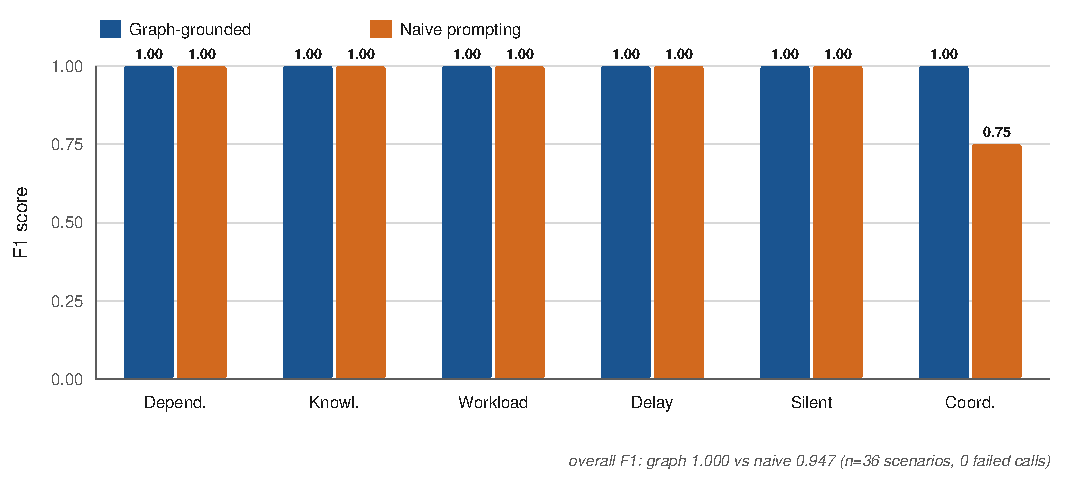
\includegraphics[width=\columnwidth]{docs/paper_figures/fig4_ablation.pdf}
\caption{Per-risk-type F1: graph-grounded vs.\ naive prompting, on identical
scenarios and identical injected ground truth.}
\label{fig:ablation}
\end{figure}

We state the resulting claim precisely rather than overclaiming: the naive baseline
is not poor (F1 0.947 is respectable), and an initial impression from inspecting
individual outputs -- that naive prompting over-reports extraneous risks -- did not
hold up under aggregate analysis: naive prompting reports a mean of 2.75 risk types
per scenario against the graph architecture's 2.42, with only 12.1\% of its claims
uncorroborated by the deterministic graph computation. The defensible claim is that
graph-grounding is \emph{no worse} on detection accuracy while being far cheaper at
scale and fully deterministic and grounded, not that naive prompting is incapable of
detecting risk on small projects.

\subsection{Live-LLM Metrics}

To assess whether the LLM narration layer stays consistent with the deterministic
computation it is meant only to explain, we measured agreement between the LLM's
narrated \texttt{risk\_level} and the deterministic fallback's verdict on identical
input, across 90 live model calls spanning all six risk types. Cohen's
$\kappa$~\cite{cohen-kappa} $= 0.9533$ ($n=37$ successful comparisons), corresponding
to ``almost perfect'' agreement on the Landis--Koch scale~\cite{landis-koch} --
direct evidence that the language model narrates rather than re-decides. Two of six
risk types (dependency, $n=14$; knowledge, $n=12$) carry most of the statistical
weight; the remainder have thin samples (as low as $n=1$) due to rate-limiting on the
evaluation account, a limitation we discuss in Section~IX. Separately, of 24
diagnosed call failures, 22 were HTTP rate-limit responses rather than genuine model
failures. Because only 24 of the 50 failures were diagnosed individually, the validity
rate over calls that actually reached the model is bounded rather than measured: 54\%
if every undiagnosed failure reached the model, 95\% if none did. We therefore report
41.1\% (37/90) as the measured end-to-end rate on this infrastructure and 54--95\% as
the range for the model's own schema validity, pending a re-run with per-call error
logging.

\section{Discussion}

The results support a precise claim, and we are careful not to extend it further: a
simple, explainable, zero-parameter graph rule matches a tuned learned model on unseen
projects, at a fraction of the token cost of naive LLM prompting, without loss of
detection accuracy in a controlled ablation, and it delivers its warning while the
sprint can still be changed. Each half of that sentence is bounded. ``Matches'' is
literal: a paired test on the held-out sprints cannot separate the two predictors
($p = 0.78$), and we do not claim the rule is more accurate -- only that the learned
model's cross-validated advantage did not cross project boundaries. The mid-sprint
result is an improvement over flagging every sprint, not over ranking by open work,
which performs comparably. This is a narrower claim than ``deterministic graph rules
are always superior to learned models'' -- the result reflects this specific problem's
structure (a low-parameter, sprint-level delay signal, evaluated with strict
project-level held-out discipline), not a general argument against learning.

\textbf{Why simplicity won here.} The negative results in Section~VII-C converge on
one explanation: with limited real-world training data (717 tuning sprints across
only nine projects) and features that are partly redundant or spuriously correlated
with the label (idle-member-ratio in particular), a model with more free parameters
had more room to fit project-specific structure that does not transfer. This is
consistent with a broader pattern in fault-prediction literature, where simple
models frequently generalize competitively against more complex
alternatives~\cite{fault-prediction-review}.

\textbf{Ethical considerations.} Because several risk types operate on
\emph{people} -- workload pressure, silent-member detection -- this system risks
being read as, or misused as, individual performance surveillance rather than
team-coordination support. We surface risk at the team level and tie every flag to
concrete, inspectable evidence specifically so findings can be contested rather than
taken as an opaque verdict on an individual; deployments should treat these signals
as prompts for a conversation, not as an automated performance assessment.

\textbf{Generalizability.} The graph schema (people, tasks, dependencies, comments,
components) is not specific to software engineering and could plausibly transfer to
other coordinated-work domains (support operations, research teams, sales
pipelines) with a different label definition; we have not tested this and state it
only as a plausible direction, not a validated one.

\section{Threats to Validity}

We list twelve threats explicitly rather than allowing them to remain implicit.
(1)~The TAWOS delay label is a proxy, since the dataset lacks a due-date field; the
30\%-unresolved-at-sprint-end definition is defensible but not canonical.
(2)~Only one of six risk types (delay) has real-world, non-synthetic validation;
structural signals (single-point-of-failure, dependency cycles, coordination) are
nearly always zero in this sprint-level reconstruction, because TAWOS issue links
span a project's entire history and rarely fall inside one sprint window, so the
other five risk types are validated only synthetically. (3)~The blocked-ratio
detector never fires on TAWOS, whose status vocabulary contains no blocked state.
(4)~AUC is weak by construction at the sprint level, since every task in a
reconstructed sprint shares one deadline. (5)~The live-LLM sample is thin and
imbalanced: the overall $\kappa$ estimate rests on $n=37$, with three of six risk
types represented by a single comparison each, and reflects a single provider, a
single model, and one rate-limited API key. (6)~We have not conducted a human
evaluation of explanation quality; grounding demonstrates that citations are real,
not that the resulting explanations are useful to a practitioner. (7)~The bootstrap
interval quantifies sampling uncertainty from one fixed split; it does not
substitute for evaluation on an independent dataset. (8)~The mid-sprint projection
does not rank sprints better than the share of work still open (AUC 0.792 versus
0.802 at the halfway checkpoint, 0.874 versus 0.881 at three-quarters); its
contribution is an early, evidence-carrying warning rather than superior
discrimination. (9)~Perfect recall in the sprint-end evaluation is structural,
guaranteed by the label definition at that evaluation point, and should not be read
as predictive skill; only the mid-sprint recall is informative. (10)~The mid-sprint
signal is deliberately inactive before a quarter of the sprint has elapsed, so no
claim is made about the earliest phase of a sprint. (11)~Two designed agents (Meeting
Intelligence, Communication Intelligence) are unimplemented because no transcript or
chat/email data source yet exists in the product -- an explicit scoping decision.
(12)~We have not conducted a longitudinal study showing that a flagged risk predicts
a real downstream outcome over subsequent weeks.

\section{Conclusion and Future Work}

We presented graph-grounded agent prompting, an architecture that separates
deterministic risk computation from language-model-based risk narration and
mechanically enforces that separation through evidence grounding. The design yields
measured, not merely claimed, efficiency (487$\times$ lower prompt cost than naive
prompting at scale) and trustworthiness (200/200 fabricated citations caught), and a
held-out real-world evaluation shows this efficiency does not cost accuracy: a
zero-parameter graph rule matches a tuned learned model on unseen projects -- a paired
test cannot separate them -- and a controlled ablation shows this is not an artifact of
an easy comparison. Projected forward from work completed so far, the same graph warns
of late sprints at their halfway point (AUC 0.792, rising to 0.874 at three-quarters),
which is where such a warning has to arrive to be worth acting on. We reported three negative
results from attempts to improve on the simple rule specifically because they
substantiate rather than undermine this claim.

Future work includes: implementing Meeting and Communication Intelligence against
the AMI Meeting Corpus and Enron Email Corpus respectively, which would additionally
strengthen validation of the coordination and silent-member risk types on real data;
a human evaluation of narration usefulness with practicing project managers;
completing fine-grained role-based access control; and a longitudinal study
connecting flagged risk to observed project outcomes.

\bibliographystyle{IEEEtran}
\begin{thebibliography}{16}

\bibitem{tawos} V. Tawosi, A. Al-Subaihin, R. Moussa, and F. Sarro, ``A versatile
dataset of agile open source software projects,'' in \emph{Proc. 19th Int. Conf.
Mining Software Repositories (MSR)}, 2022, doi: 10.1145/3524842.3528029.

\bibitem{networkx} A. Hagberg, P. Swart, and D. S Chult, ``Exploring network
structure, dynamics, and function using NetworkX,'' in \emph{Proc. 7th Python in
Science Conf. (SciPy)}, 2008, pp. 11--15.

\bibitem{bootstrap} B. Efron, ``Bootstrap methods: Another look at the jackknife,''
\emph{Annals of Statistics}, vol. 7, no. 1, pp. 1--26, 1979.

\bibitem{metagpt} S. Hong \emph{et al.}, ``MetaGPT: Meta programming for a
multi-agent collaborative framework,'' in \emph{Proc. Int. Conf. Learning
Representations (ICLR)}, 2024, arXiv:2308.00352.

\bibitem{chatdev} C. Qian \emph{et al.}, ``ChatDev: Communicative agents for
software development,'' in \emph{Proc. 62nd Annu. Meeting Assoc. Computational
Linguistics (ACL)}, 2024, arXiv:2307.07924.

\bibitem{agentbench} X. Liu \emph{et al.}, ``AgentBench: Evaluating LLMs as
agents,'' in \emph{Proc. Int. Conf. Learning Representations (ICLR)}, 2024,
arXiv:2308.03688.

\bibitem{react} S. Yao \emph{et al.}, ``ReAct: Synergizing reasoning and acting in
language models,'' in \emph{Proc. Int. Conf. Learning Representations (ICLR)},
2023, arXiv:2210.03629.

\bibitem{shap} S. M. Lundberg and S.-I. Lee, ``A unified approach to interpreting
model predictions,'' in \emph{Advances in Neural Information Processing Systems
(NeurIPS)}, vol. 30, 2017.

\bibitem{lime} M. T. Ribeiro, S. Singh, and C. Guestrin, ```Why should I trust
you?': Explaining the predictions of any classifier,'' in \emph{Proc. 22nd ACM
SIGKDD Int. Conf. Knowledge Discovery and Data Mining (KDD)}, 2016, pp.
1135--1144.

\bibitem{jiarpakdee} J. Jiarpakdee, C. Tantithamthavorn, H. K. Dam, and J. Grundy,
``An empirical study of model-agnostic techniques for defect prediction models,''
\emph{IEEE Trans. Software Engineering}, vol. 48, no. 1, pp. 166--185, 2022.

\bibitem{rag} P. Lewis \emph{et al.}, ``Retrieval-augmented generation for
knowledge-intensive NLP tasks,'' in \emph{Advances in Neural Information
Processing Systems (NeurIPS)}, vol. 33, 2020.

\bibitem{hallucination-survey} Z. Ji \emph{et al.}, ``Survey of hallucination in
natural language generation,'' \emph{ACM Computing Surveys}, vol. 55, no. 12, pp.
1--38, 2023.

\bibitem{gnn-survey} J. Zhou \emph{et al.}, ``Graph neural networks: A review of
methods and applications,'' \emph{AI Open}, vol. 1, pp. 57--81, 2020.

\bibitem{cohen-kappa} J. Cohen, ``A coefficient of agreement for nominal scales,''
\emph{Educational and Psychological Measurement}, vol. 20, no. 1, pp. 37--46, 1960.

\bibitem{landis-koch} J. R. Landis and G. G. Koch, ``The measurement of observer
agreement for categorical data,'' \emph{Biometrics}, vol. 33, no. 1, pp. 159--174,
1977.

\bibitem{fault-prediction-review} T. Hall, S. Beecham, D. Bowes, D. Gray, and S.
Counsell, ``A systematic literature review on fault prediction performance in
software engineering,'' \emph{IEEE Trans. Software Engineering}, vol. 38, no. 6,
pp. 1276--1304, 2012.

\end{thebibliography}

\end{document}
